\documentclass{standalone}
\title{}
\date{}
\author{}
\usepackage{amsmath}
\usepackage{amssymb}
\usepackage{algorithm}
\usepackage[noend]{algorithmic}
\usepackage{tikz}
\usetikzlibrary{decorations.pathreplacing,angles,quotes}
\begin{document}

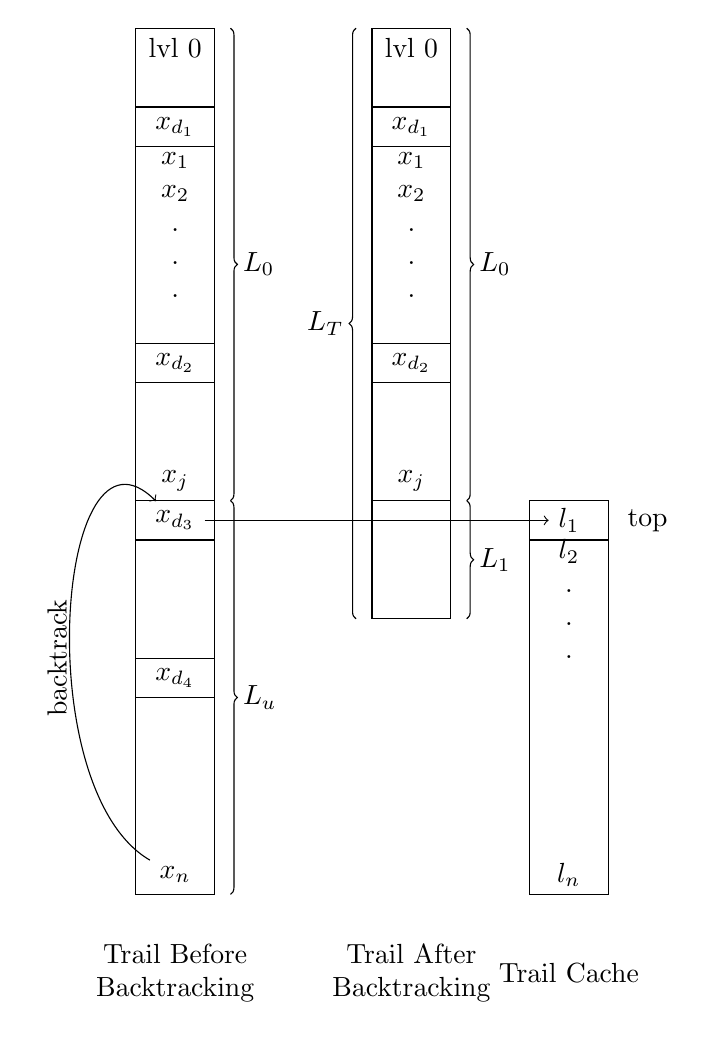
\begin{tikzpicture}
\draw (0, 10) rectangle (1, 11);
\draw (0, 9.5) rectangle (1, 10);
\draw (0, 7) rectangle (1, 9.5);
\draw (0, 6.5) rectangle (1, 7);
\draw (0, 3) rectangle (1, 6.5);
\draw (0, 4.5) rectangle (1, 5);
\draw (0, 2.5) rectangle (1, 3);
\draw (0, 0) rectangle (1, 2.5);
\node[align=center] at (0.5, 10.75) {lvl 0};
\node[align=center] at (0.5, 9.75) {$x_{d_1}$};
\node[align=center] at (0.5, 8.5) {$x_1$ \\ $x_2$ \\ . \\ . \\ .};
\node[align=center] at (0.5, 6.75) {$x_{d_2}$};
\node[align=center] at (0.5, 5.25) {$x_j$};
\node[align=center] (A) at (0.5, 4.75) {$x_{d_3}$};
\node[align=center] at (0.5, 2.75) {$x_{d_4}$};
\node[align=center] (C) at (0.5, 0.25) {$x_n$};

\draw (3, 10) rectangle (4, 11);
\draw (3, 9.5) rectangle (4, 10);
\draw (3, 7) rectangle (4, 9.5);
\draw (3, 6.5) rectangle (4, 7);
\draw (3, 5) rectangle (4, 6.5);
\draw (3, 6.5) rectangle (4, 3.5);
\draw (5, 4.5) rectangle (6, 5);
\draw (5, 0) rectangle (6, 4.5);
%\draw (5, 2.5) rectangle (6, 3);
%\draw (5, 0) rectangle (6, 2.5);
\node[align=center] at (3.5, 10.75) {lvl 0};
\node[align=center] at (3.5, 9.75) {$x_{d_1}$};
\node[align=center] at (3.5, 8.5) {$x_1$ \\ $x_2$ \\ . \\ . \\ .};
\node[align=center] at (3.5, 6.75) {$x_{d_2}$};
\node[align=center] at (3.5, 5.25) {$x_j$};
\node[align=center] (B) at (5.5, 4.75) {$l_1$};
\node[align=center] at (5.5, 3.75) {$l_2$ \\ . \\ . \\ .};
%\node[align=center] at (5.5, 2.75) {$l_k$};
\node[align=center] at (5.5, 0.25) {$l_n$};
\node[align=center] at (6.5, 4.75) {top};

\draw[decoration={brace,raise=20pt},decorate] (0.5, 5) -- node[right=21pt] {$L_u$} (0.5, 0);
\draw[decoration={brace,raise=20pt},decorate] (0.5, 11) -- node[right=21pt] {$L_0$} (0.5, 5);
\draw[decoration={brace,raise=20pt},decorate] (3.5, 11) -- node[right=21pt] {$L_0$} (3.5, 5);
\draw[decoration={brace,raise=20pt},decorate] (3.5, 5) -- node[right=21pt] {$L_1$} (3.5, 3.5);
\draw[decoration={brace,mirror,raise=20pt},decorate] (3.5, 11) -- node[left=21pt] {$L_T$} (3.5, 3.5);

\node[align=center] at (0.5, -1) {Trail Before \\ Backtracking};
\node[align=center] at (3.5, -1) {Trail After \\ Backtracking};
\node[align=center] at (5.5, -1) {Trail Cache};
\draw[->] (A) -- (B);
\draw[->] (C) to [out=150] (A) node[rotate=90] at (-1,3) {backtrack};
\end{tikzpicture}
\end{document}